\documentclass[a4paper]{article}
\usepackage{graphicx}
\begin{document}
\section{JSON}
\subsection{Definisi JSON}
JSON atau JavaScript Object Notation adalah salah satu bentuk format yang ringkas untuk melakukan pertukaran sebuah data di dalam computer. JSON sendiri berbasis teks dan mudah untuk dibaca oleh manusia serta dapat digunakan untuk representasi struktur data sederhana JSON juga dapat digunakan untuk proses transmisi data terstruktur melalui media koneksi jaringan yang disebut Serialisasi.
\subsection{Definisi JSON}
JSON atau (JavaScript Object Notation) merupakan  bagian  dari  sebuah bahasa  pemrograman web  JavaScript.  JSON juga merupakan format teks yang semuanya bersifat independen tetapi menggunakan konvensi yang  hampir sama  dengan  bahasa  pemrograman  dari  parent-C,  termasuk juga dengan  bahasa C,  Java,  Java Script,  Perl, Python,  dan lain sebagainya.  Kelebihan  inilah  yang  membuat  JSON  menjadi  sebuah  bahasa yang disebut  data-interchange yang ideal.
\subsection{Struktur pada JSON}
JSON memiliki 2 struktur,yaitu:
1.	Kumpulan pasangan nama/nilai.
Dalam beberapa Bahasa pemrograman, ini biasanya sering disebut seperti objek, rekaman, struktur, kamus, tabel hash, daftar berkunci atau array assosiatif.
2.	Daftar nilai terurutkan.
Dalam kebanyakan Bahasa pemrograman, ini biasanya sering disebut seperti array, vektor, daftar, atau urutan.
Struktur data tersebut sering kali disebut sebagai struktur data universal. Semua bahasa pemrograman modern mendukung struktur data tersebut dalam bentuk yang sama maupun berbeda.
\subsection{Pengertian Lain Dari JSON}
JSON atau biasa dilafalkan dengan “Jason” merupakan singkatan dari JavaScript Object Notation adalah suatu format ringkas pertukaran data computer. Format Json berbasis teks dan mudah dibaca-manusia serta digunakan untuk merepresentasikan struktur data sederhana dan larik asosiatif. JSON juga seringkali digunakan untuk transmisi datayang  terstruktur melalui suatu koneksi jaringan pada suatu proses yang disebut serialisasi.
\subsection{JSON}
Secara umum Penggunaan JSON terdiri dari 2 fungsi encode dan decode.  JSON decode Merupakan proses untuk  memperoleh nilai dari sutu variable dengan berkas JSON array. Method json encode akan mengubah nilai dari variabel  menjadi suatu format yang dapat dibaca sebagai JSON array. method json decode  akan mengekstrak nilai dari variabel JSON array  menjadi suatu nilai output.
\subsection{JSON}
Kelebihan utama dari JSON dibandingkan dengan XML adalah dari bentuk sisi dan ukuran file, JSON memiliki ukuran yang relatif  lebih kecil dibandingkan dengan file dari XML. File yang berukuran keciil sanagat penting untuk web service yang akan dibuat dikarenakan nantinya data akan diakses oleh aplikasi mobile yang membutuhkan respon cepat.
\subsection{JSON}
YAML mempunyai fitur tambahan yang sangat bagus seperti komentar, aliasing dan anchoring.  Dibandingkan dari YAML, JSON yang agak terbatas. Tetapi, JSON lebih banyak digunakan dan didukung. Salah satu alasan yang kuatnya adalah lebih cepat terhubung dan deserialize, yang merupakan penentu kunci untuk berkomunikasi antara klien dan server.
•	Gunakanlah JSON untuk komunikasi antara klien dan server.
•	Gunakanlah YAML untuk file konfigurasi karena YAML benar-benar dapat dibaca manusia.
\subsection{JSON}
XML merupakan format transfer data sejak lama, tetapi beberapa tahun terakhir, JSON meyalip posisi XML. Kelebihan JSON dibandingkan dengan XML sebagai berikut:\\
1.	Ukuran format JSON lebih kecil dibandingkan dengan fortmat XML, dan berefek kepada transfer data lebih cepat dan lebih hemat resource.\\
2.	JSON merupakan format data dalam bahasa pemrograman Javascript, yang artinya jika data dari server di kirim ke klien , dan klien menggunakan javascript, maka tidak perlu library tambahan untuk memprosesnya.\\
3.	Dibandingkan dengan XML, format transfer data JSON lebih sederhana.

\section{YAML}
\subsection{Definisi YAML}
YAML atau YAML Ain't Markup Language adalah sebuah standar yang sudah umum untuk digunakan proses Serialisasi data dalam semua Bahasa pemrograman. YAML dapat memberikan representasi data dengan bentuk yang lebih sederhana. Salah satu bentuk penyederhanaan nya adalah dengan menghilangkan tanda {} dan tanda []. YAML sendiri juga memiliki fitur yang tidak dimiliki oleh JSON.
\begin{figure}[ht]
\centerline{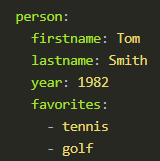
\includegraphics[scale=1]{../figures/5SC.png} }

\caption{Contoh Source Code} 
\label{Sc}
\end{figure}

Pada gambar \ref{Sc} dijelaskan tentang Contoh Source Code.

\subsection{Definisi Lain dari YAML}
YAML merupakan format serial data yang dapat dibaca oleh manusia yang mengambil beberapa bahas apemrograman seperti XML, C, Python, serta format email seperti yang recantum dalam RFC 2822. Pengusul YAML adalah Clark Evans pada tahun2001 silam. Clark merancang format ini bersama dengan Ingy döt Net dan Oren Ben-Kiki. YAML pula tersedia dalam beberapa Bahasa dan script pemrograman.
\subsection{YAML}
YAML mengintegrasikan dan membangun berdasarkan konsep yang dijelaskan oleh bahasa C, Java, Perl, Python, Ruby, MAIL,  HTML, MIME, URI, XML, SAX, SOAP, dan JSON.
Sintak YAML motivated oleh Internet Mail  dan tetap sebagian kompatibel dengan standar itu. selanjutnya, meminjam dari MIME , produksi tingkat atas YAML adalah aliran dokumen independen, ideal untuk pesan berbasissistem pemrosesan terdistribusi
\subsection{Definisi YAML}
Pada saat awal-awal perkembangan, YAML diartikan dari banyak orang adalah sebuah singkatan yaitu "Yet Another Markup Language". Namun seiring berkembangnya zaman, untuk memberitahu tujuannya lebih jauh yang terfokus pada data dan bukan markah dokumen, akhirnya singkatan YAML diubah menjadi "YAML Ain't a Markup Language." YAML tersedia untuk beberapa Bahasa dan skrip pemrograman.
\subsection{YAML}
Dari pembahasan di atas, yang telah membahas tentang JSON atau JavaScript Object Notation dan YAML atau YAML Aint Markup Language. Berdasarkan pembahasan di atas dapat di temukan perbedaan antara keduanya. Berikut adalah beberapa perbedaan yang dapat kami kemukakan:
Berikut adalah tabel \ref{table:perbedaan} perbedaan JSON dan YAML.
\begin{table}[h]
\caption{Perbedaan JSON dan YAML}

\centering
\begin{tabular}{ccc}
\hline
&JSON&YAML\\
\hline
Kegunaan&Cocok untuk Format Serialisasi&Cocok untuk konfigurasi\\
\hline
Fitur&tidak memiliki komentar, aliasing&memiliki komentar, aliasing \\
&dan anchoring, dan  mergering& dan anchoring, dan  mergering\\
\hline
\end{tabular}
\label{table:perbedaan}
\end{table}

\subsection{Kelebihan JSON}
JSON tentunya memiliki beberapa kelebihan, berikut Kelebihan JSON :
1.	Mudah dibaca dan ditulis oleh computer dan manusia.
2.	Hampir semua Bahasa pemrogaraman menyediakan pustaka atau fungsi uang memudahkan untuk membaca dan membuat struktur JSON.
3.	JSON mudah di disusun pada struktur data yang digunakan oleh sebagain besar Bahasa pemrograman terkait yang memiliki data berupa integer, string, Boolean, null, array, dan associative array.

\subsection{Format Data JSON}
Pada JSON format datanya mempunyai aturan sebagai berikut :
1. Object merupakan satu kesatuan nama/nilai yang tidak berurutan. Penulisan biasanya diawali dengan tanda { (dan diakhiri dengan tanda } .
Pada setiap nama selalu diikuti oleh tanda : dan nilai dipisahkan oleh tanda , .
2.  Array merupakan kumpulan nilai yang beraturan. Penulisan biasanya diawali dengan tanda [ dan diakhiri dengan tanda ]
3. Nilai dapat berupa string atau number, TRUE atau FALSE atau NULL, sebuah object atau sebuah array. Strukturnya dapat ditulis menggunakan metode bersarang
4. String merupakan serangkaian atau urutan karakter unicode yang ada di dalam tanda kutip atau hanya berisi karakter kosong, penulisannya menggunakan tanda \  untuk escape.

\subsection{Alasan JSON}
JSON atau JavaScript Object Notation salah satu pertukaran data yang sering digunakan. JSON juga merupakan salah satu bentuk format teks yang bersifat independen atau berdiri sendiri namun menggunakan konversi data yang sangat familiar dengan beberapa Bahasa pemrograman seperti:

\begin{enumerate}
\item C
\item C++
\item C\#
\item Javascript
\item Java
\item Perl
\item Python

\end{enumerate}
Dari pembahasan diatas itulah mengapa JSON disebut sebagai Bahasa interpreter-data yang sering digunakan.
\subsection{Manfaat JSON}
1.	Pengguna dapat melakukan klik pada gambar thumbnail pada sebuah produk yang dijual pada toko online
2.	Setelah itu cript Javascript dijalankan di browser, melakukan Ajax request ke script PHP dan akan dijalankan pada server lalu melemparkan ID dari produk yang dipilih
3.	Selanjutnya script PHP mengambil data nama produk, deskripsi, harga dan info lain dari database. Kemudian data tersebut diubah dalam bentuk JSON dan dikirim kembali ke browser.
4.	Javascript yang jalan pada browser kemudian membaca format JSON dan menampilkan detail informasi pada pengguna.
5.	Saat proses tersebut terjadi, browser pengguna tidak perlu melakukan reload atau berganti halaman. Semuanya telah terjadi di background.

\subsection{Perbandingan Antara XML dan JSON}
XML memiliki kemiripan dengan JSON, tetapi XML lebih membutuhkan lebih banyak teks sehingga isinya lebih panjang dan lebih lama untuk dibaca dan ditulis dibandingkan dengan JSON. XML hanya bisa dibaca oleh XML parser. Berbeda dengan JSON yang bisa dibaca dengan mudah menggunakan fungsi standar. Selain itu, XML tidak bisa menggunakan array seperti JSON.

\subsection{sejarah YAML}
Sejarah YAML di usulkan oleh Clark Evans tahun 2001. Lalu di desain sedemikian rupa secara bersama-sama oleh Ingy dot Net dan Oren Ben Kiki. Suatu ketika, format ini di desain ulang berdasarkan pengalaman dan dikembangkan serta di diskusikan bersama anggota sml-dev internet, masih bisa untuk diperbaharui berdasarkan masukkan dari para penggunanya.

\subsection{Kelebihan AJAX}
Jika sebelumnya kita membahas tentang kelebihan JSON, maka kali ini kita akan membahas tentang kelebihan AJAX. AJAX atau singkatan dari Asynchronus JavaScript and XML merupakan sebuah teknologi developing web application interaktif dan dinamis yang menawarkan pengalaman bagi user yang sangat baik. Berikut kelebihan dari AJAX :
1.	Meningkatan User Experience (UX)/ Pengalaman Pengguna.
2.	Meningkatkan produktivitas terhadap pengguna.
3.	Mengurangi penggunaan bandwith dan meningkatkan kecepatan.
4.	Meningkatkan compatibility.
5.	Mendukung proses Asynchronus.
6.	Mengurangi hit server dan beban jaringan.
7.	Navigasi menjadi lebih mudah.
8.	Ada pemisahan antara data, style, format, dan fungsi.

\subsection{Kekurangan AJAX}
Ajax tidak hanya memiliki kelebihan, ia juga memiliki kekurangan. Kekurangan yang dimiliki oleh ajax adalah sebagai berikut :
1.	Kompatibilitas browser
2.	Kerawanan
3.	Peningkatan beban web server
4.	Sulit di bookmark/favorite
5.	Tidak bagus untuk SEO
6.	Kurang dukungan editor
7.	Waktu Pengembangan jadi lebih lama
8.	Web analytic tidak maksimal

\subsection{Implementasi YAML}
Implementasi YAML atau YAML Ain’t Markup Language sangat cocok untuk konfigurasi file.
Berikut adalah beberapa implementasi dari YAML :
\begin{itemize}
\item YAML.load berfungsi untuk memparsing string atau aliran sebuah file yang berisi dokumen YAML.
\item YAML.dump berfungsi untuk memakai objek 
\item Modul YAML dapat membuat Salinan data identik semantis dari objek yang asli lalu di lakukan proses serialisasi.

\end{itemize}

\end{document}
